\documentclass[]{article}
\usepackage{lmodern}
\usepackage{amssymb,amsmath}
\usepackage{ifxetex,ifluatex}
\usepackage{fixltx2e} % provides \textsubscript
\ifnum 0\ifxetex 1\fi\ifluatex 1\fi=0 % if pdftex
  \usepackage[T1]{fontenc}
  \usepackage[utf8]{inputenc}
\else % if luatex or xelatex
  \ifxetex
    \usepackage{mathspec}
  \else
    \usepackage{fontspec}
  \fi
  \defaultfontfeatures{Ligatures=TeX,Scale=MatchLowercase}
\fi
% use upquote if available, for straight quotes in verbatim environments
\IfFileExists{upquote.sty}{\usepackage{upquote}}{}
% use microtype if available
\IfFileExists{microtype.sty}{%
\usepackage{microtype}
\UseMicrotypeSet[protrusion]{basicmath} % disable protrusion for tt fonts
}{}
\usepackage[margin=1in]{geometry}
\usepackage{hyperref}
\hypersetup{unicode=true,
            pdftitle={Michigan Home Prices},
            pdfborder={0 0 0},
            breaklinks=true}
\urlstyle{same}  % don't use monospace font for urls
\usepackage{color}
\usepackage{fancyvrb}
\newcommand{\VerbBar}{|}
\newcommand{\VERB}{\Verb[commandchars=\\\{\}]}
\DefineVerbatimEnvironment{Highlighting}{Verbatim}{commandchars=\\\{\}}
% Add ',fontsize=\small' for more characters per line
\usepackage{framed}
\definecolor{shadecolor}{RGB}{248,248,248}
\newenvironment{Shaded}{\begin{snugshade}}{\end{snugshade}}
\newcommand{\KeywordTok}[1]{\textcolor[rgb]{0.13,0.29,0.53}{\textbf{#1}}}
\newcommand{\DataTypeTok}[1]{\textcolor[rgb]{0.13,0.29,0.53}{#1}}
\newcommand{\DecValTok}[1]{\textcolor[rgb]{0.00,0.00,0.81}{#1}}
\newcommand{\BaseNTok}[1]{\textcolor[rgb]{0.00,0.00,0.81}{#1}}
\newcommand{\FloatTok}[1]{\textcolor[rgb]{0.00,0.00,0.81}{#1}}
\newcommand{\ConstantTok}[1]{\textcolor[rgb]{0.00,0.00,0.00}{#1}}
\newcommand{\CharTok}[1]{\textcolor[rgb]{0.31,0.60,0.02}{#1}}
\newcommand{\SpecialCharTok}[1]{\textcolor[rgb]{0.00,0.00,0.00}{#1}}
\newcommand{\StringTok}[1]{\textcolor[rgb]{0.31,0.60,0.02}{#1}}
\newcommand{\VerbatimStringTok}[1]{\textcolor[rgb]{0.31,0.60,0.02}{#1}}
\newcommand{\SpecialStringTok}[1]{\textcolor[rgb]{0.31,0.60,0.02}{#1}}
\newcommand{\ImportTok}[1]{#1}
\newcommand{\CommentTok}[1]{\textcolor[rgb]{0.56,0.35,0.01}{\textit{#1}}}
\newcommand{\DocumentationTok}[1]{\textcolor[rgb]{0.56,0.35,0.01}{\textbf{\textit{#1}}}}
\newcommand{\AnnotationTok}[1]{\textcolor[rgb]{0.56,0.35,0.01}{\textbf{\textit{#1}}}}
\newcommand{\CommentVarTok}[1]{\textcolor[rgb]{0.56,0.35,0.01}{\textbf{\textit{#1}}}}
\newcommand{\OtherTok}[1]{\textcolor[rgb]{0.56,0.35,0.01}{#1}}
\newcommand{\FunctionTok}[1]{\textcolor[rgb]{0.00,0.00,0.00}{#1}}
\newcommand{\VariableTok}[1]{\textcolor[rgb]{0.00,0.00,0.00}{#1}}
\newcommand{\ControlFlowTok}[1]{\textcolor[rgb]{0.13,0.29,0.53}{\textbf{#1}}}
\newcommand{\OperatorTok}[1]{\textcolor[rgb]{0.81,0.36,0.00}{\textbf{#1}}}
\newcommand{\BuiltInTok}[1]{#1}
\newcommand{\ExtensionTok}[1]{#1}
\newcommand{\PreprocessorTok}[1]{\textcolor[rgb]{0.56,0.35,0.01}{\textit{#1}}}
\newcommand{\AttributeTok}[1]{\textcolor[rgb]{0.77,0.63,0.00}{#1}}
\newcommand{\RegionMarkerTok}[1]{#1}
\newcommand{\InformationTok}[1]{\textcolor[rgb]{0.56,0.35,0.01}{\textbf{\textit{#1}}}}
\newcommand{\WarningTok}[1]{\textcolor[rgb]{0.56,0.35,0.01}{\textbf{\textit{#1}}}}
\newcommand{\AlertTok}[1]{\textcolor[rgb]{0.94,0.16,0.16}{#1}}
\newcommand{\ErrorTok}[1]{\textcolor[rgb]{0.64,0.00,0.00}{\textbf{#1}}}
\newcommand{\NormalTok}[1]{#1}
\usepackage{graphicx,grffile}
\makeatletter
\def\maxwidth{\ifdim\Gin@nat@width>\linewidth\linewidth\else\Gin@nat@width\fi}
\def\maxheight{\ifdim\Gin@nat@height>\textheight\textheight\else\Gin@nat@height\fi}
\makeatother
% Scale images if necessary, so that they will not overflow the page
% margins by default, and it is still possible to overwrite the defaults
% using explicit options in \includegraphics[width, height, ...]{}
\setkeys{Gin}{width=\maxwidth,height=\maxheight,keepaspectratio}
\IfFileExists{parskip.sty}{%
\usepackage{parskip}
}{% else
\setlength{\parindent}{0pt}
\setlength{\parskip}{6pt plus 2pt minus 1pt}
}
\setlength{\emergencystretch}{3em}  % prevent overfull lines
\providecommand{\tightlist}{%
  \setlength{\itemsep}{0pt}\setlength{\parskip}{0pt}}
\setcounter{secnumdepth}{0}
% Redefines (sub)paragraphs to behave more like sections
\ifx\paragraph\undefined\else
\let\oldparagraph\paragraph
\renewcommand{\paragraph}[1]{\oldparagraph{#1}\mbox{}}
\fi
\ifx\subparagraph\undefined\else
\let\oldsubparagraph\subparagraph
\renewcommand{\subparagraph}[1]{\oldsubparagraph{#1}\mbox{}}
\fi

%%% Use protect on footnotes to avoid problems with footnotes in titles
\let\rmarkdownfootnote\footnote%
\def\footnote{\protect\rmarkdownfootnote}

%%% Change title format to be more compact
\usepackage{titling}

% Create subtitle command for use in maketitle
\newcommand{\subtitle}[1]{
  \posttitle{
    \begin{center}\large#1\end{center}
    }
}

\setlength{\droptitle}{-2em}

  \title{Michigan Home Prices}
    \pretitle{\vspace{\droptitle}\centering\huge}
  \posttitle{\par}
    \author{}
    \preauthor{}\postauthor{}
    \date{}
    \predate{}\postdate{}
  

\begin{document}
\maketitle

\section{Step 1: Ask a research
question}\label{step-1-ask-a-research-question}

\begin{enumerate}
\def\labelenumi{\arabic{enumi}.}
\tightlist
\item
  I want to predict how much should I expect to pay for a home. What
  explanatory variables might explain variation in home prices?
\end{enumerate}

SOLUTION: explanatory variables might include: location, square footage,
number of baths/beds

\section{Step 2: Design a study and collect
data}\label{step-2-design-a-study-and-collect-data}

\begin{enumerate}
\def\labelenumi{\arabic{enumi}.}
\setcounter{enumi}{1}
\tightlist
\item
  ID the observational units and the response variable of interest. Is
  the response variable quantitative or categorical? What kinds of
  graphs and numerical summaries can you use to explore these data?
\end{enumerate}

\begin{Shaded}
\begin{Highlighting}[]
\KeywordTok{library}\NormalTok{(tidyverse)}
\NormalTok{home.data<-}\KeywordTok{read.table}\NormalTok{(}\StringTok{"http://www.isi-stats.com/isi2/data/homeprices.txt"}\NormalTok{,}\DataTypeTok{header=}\NormalTok{T, }\DataTypeTok{fill=}\NormalTok{T)}
\KeywordTok{head}\NormalTok{(home.data)}
\end{Highlighting}
\end{Shaded}

\begin{verbatim}
##   sqft price.1000      lake
## 1 2700      639.9 lakefront
## 2 3353      898.0 lakefront
## 3 1600      410.0 lakefront
## 4 1740      529.9 lakefront
## 5 1907      495.0 lakefront
## 6 3262      749.9 lakefront
\end{verbatim}

SOLUTION: Observational units: homes north of Lake Macatawa in Michigan
Response variable of interest: sale price Response variable is
quantitative Can use a bar graph, histogram, mosaic graph, and scatter
plot; also use descriptive statistics

\section{Step 3: Explore the data}\label{step-3-explore-the-data}

\begin{enumerate}
\def\labelenumi{\arabic{enumi}.}
\setcounter{enumi}{2}
\tightlist
\item
  Describe the shape of the home prices in this sample
\end{enumerate}

\begin{Shaded}
\begin{Highlighting}[]
\NormalTok{home.data }\OperatorTok
\StringTok{  }\KeywordTok{ggplot}\NormalTok{(}\KeywordTok{aes}\NormalTok{(}\DataTypeTok{x=}\NormalTok{price.}\DecValTok{1000}\NormalTok{)) }\OperatorTok{+}
\StringTok{    }\KeywordTok{geom_histogram}\NormalTok{(}\DataTypeTok{binwidth =} \DecValTok{100}\NormalTok{)}
\end{Highlighting}
\end{Shaded}

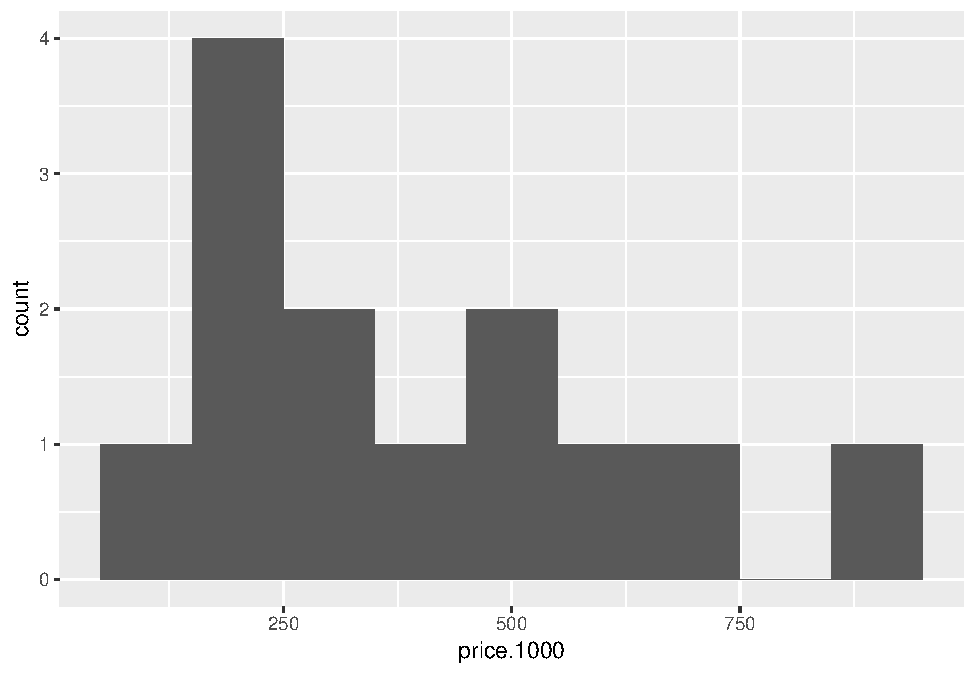
\includegraphics{Michigan_Home_Prices_files/figure-latex/unnamed-chunk-2-1.pdf}

\begin{Shaded}
\begin{Highlighting}[]
\KeywordTok{summary}\NormalTok{(home.data}\OperatorTok{$}\NormalTok{price.}\DecValTok{1000}\NormalTok{)}
\end{Highlighting}
\end{Shaded}

\begin{verbatim}
##    Min. 1st Qu.  Median    Mean 3rd Qu.    Max. 
##   119.0   210.0   324.9   408.1   529.9   898.0
\end{verbatim}

SOLUTION: The distribution of home prices in this samples is skewed to
the right (more values below the mean than above the mean)

\begin{enumerate}
\def\labelenumi{\arabic{enumi}.}
\setcounter{enumi}{3}
\tightlist
\item
  If we want to estimate a typical home price, would the mean be
  reasonable to use?
\end{enumerate}

SOLUTION: No, because the data is skewed right, the mean would
over-predict a typical home price. The median would be more appropriate
(mean should only be used when the distribution is symmetric)

\begin{enumerate}
\def\labelenumi{\arabic{enumi}.}
\setcounter{enumi}{4}
\tightlist
\item
  Do you think the mean is larger or smaller than the median.
\end{enumerate}

SOLUTION: Clearly larger (skewed right and from summary statistics)

\begin{enumerate}
\def\labelenumi{\arabic{enumi}.}
\setcounter{enumi}{5}
\tightlist
\item
  What is the standard deviation of the home prices? What are the units?
  Interpret this value. What are possible explanations for this
  variation?
\end{enumerate}

\begin{Shaded}
\begin{Highlighting}[]
\KeywordTok{sd}\NormalTok{(home.data}\OperatorTok{$}\NormalTok{price.}\DecValTok{1000}\NormalTok{)}
\end{Highlighting}
\end{Shaded}

\begin{verbatim}
## [1] 240.9228
\end{verbatim}

SOLUTION: Standard deviation is 240.9228; in other words, the typical
distance of a home is \$240,920 away from the mean. This will not
provide an accurate predication of home prices. Possible explanations
are size and location.

\begin{enumerate}
\def\labelenumi{\arabic{enumi}.}
\setcounter{enumi}{6}
\tightlist
\item
  The first home in the data set sold for \$639,000 - if we had used the
  mean to predict that price, how far off would we have been?
\end{enumerate}

\begin{Shaded}
\begin{Highlighting}[]
\DecValTok{639}\OperatorTok{-}\KeywordTok{mean}\NormalTok{(home.data}\OperatorTok{$}\NormalTok{price.}\DecValTok{1000}\NormalTok{)}
\end{Highlighting}
\end{Shaded}

\begin{verbatim}
## [1] 230.9385
\end{verbatim}

We would have been \$230,938.50 below the actual price

\begin{enumerate}
\def\labelenumi{\arabic{enumi}.}
\setcounter{enumi}{7}
\tightlist
\item
  Using the mean as our prediction, did we over-predict or under-predict
  the prices of the first house? (Is the residual positive or negative?)
\end{enumerate}

SOLUTION: We under predicted, so the residual is positive (actual -
predicted)

\begin{enumerate}
\def\labelenumi{\arabic{enumi}.}
\setcounter{enumi}{8}
\tightlist
\item
  How many residuals are positive and how many are negative?
\end{enumerate}

\begin{Shaded}
\begin{Highlighting}[]
\NormalTok{model.home.mean =}\StringTok{ }\KeywordTok{lm}\NormalTok{(price.}\DecValTok{1000} \OperatorTok{~}\StringTok{ }\DecValTok{1}\NormalTok{, }\DataTypeTok{data =}\NormalTok{ home.data)}
\NormalTok{model.home.mean.res =}\StringTok{ }\KeywordTok{resid}\NormalTok{(model.home.mean)}
\KeywordTok{plot}\NormalTok{(home.data}\OperatorTok{$}\NormalTok{price.}\DecValTok{1000}\NormalTok{, model.home.mean.res)}
\end{Highlighting}
\end{Shaded}

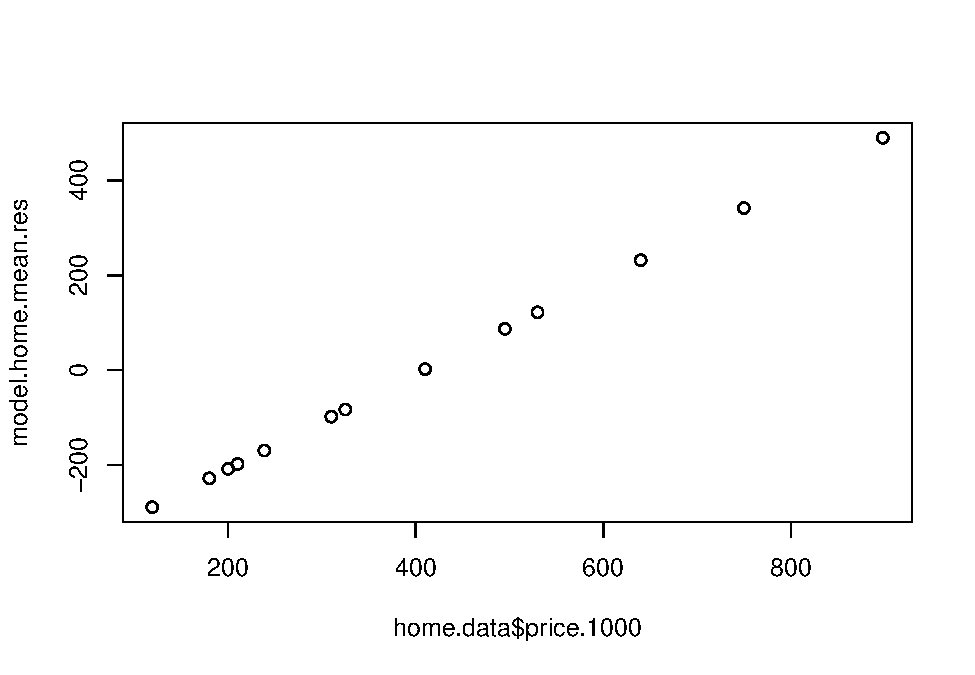
\includegraphics{Michigan_Home_Prices_files/figure-latex/unnamed-chunk-5-1.pdf}

6 are positive (over-predicted) and 7 are negative (under-predicted)

\begin{enumerate}
\def\labelenumi{\arabic{enumi}.}
\setcounter{enumi}{9}
\tightlist
\item
  Describe the association between home price and square footage
  (strength, direction, linearity). Does the association behave as you
  would have predicted? Explain
\end{enumerate}

\begin{Shaded}
\begin{Highlighting}[]
\NormalTok{home.data }\OperatorTok
\StringTok{  }\KeywordTok{ggplot}\NormalTok{(}\KeywordTok{aes}\NormalTok{(}\DataTypeTok{x=}\NormalTok{sqft, }\DataTypeTok{y=}\NormalTok{price.}\DecValTok{1000}\NormalTok{)) }\OperatorTok{+}
\StringTok{  }\KeywordTok{geom_point}\NormalTok{()}
\end{Highlighting}
\end{Shaded}

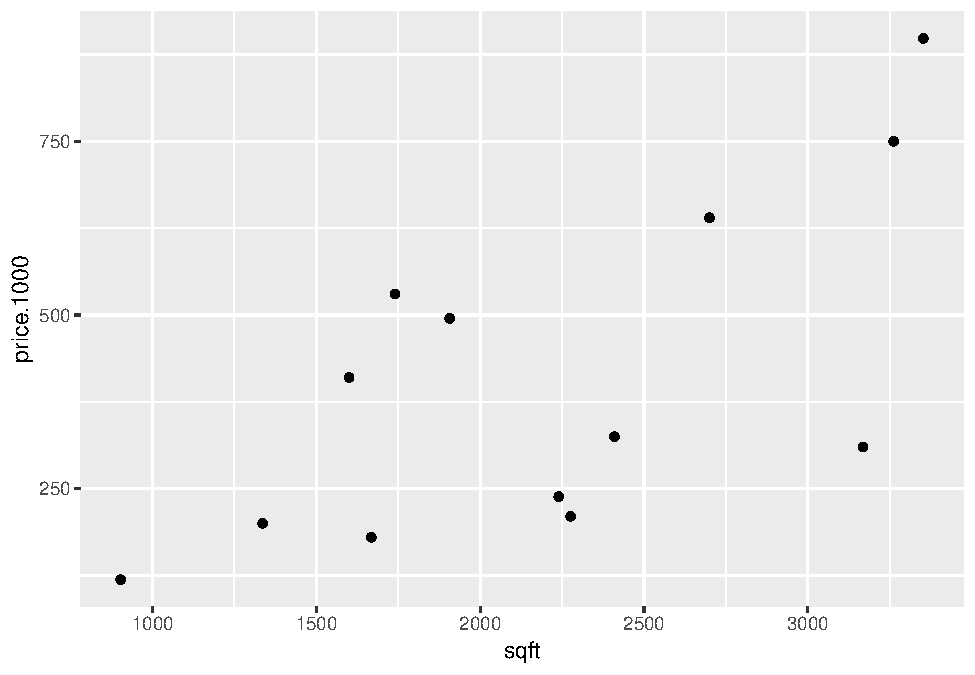
\includegraphics{Michigan_Home_Prices_files/figure-latex/unnamed-chunk-6-1.pdf}

\begin{Shaded}
\begin{Highlighting}[]
\NormalTok{model.home.}\DecValTok{1}\NormalTok{ =}\StringTok{ }\KeywordTok{lm}\NormalTok{(price.}\DecValTok{1000} \OperatorTok{~}\StringTok{ }\NormalTok{sqft, }\DataTypeTok{data =}\NormalTok{ home.data)}
\KeywordTok{summary}\NormalTok{(model.home.}\DecValTok{1}\NormalTok{)}
\end{Highlighting}
\end{Shaded}

\begin{verbatim}
## 
## Call:
## lm(formula = price.1000 ~ sqft, data = home.data)
## 
## Residuals:
##     Min      1Q  Median      3Q     Max 
## -304.70 -128.44  -13.74  128.98  244.04 
## 
## Coefficients:
##              Estimate Std. Error t value Pr(>|t|)  
## (Intercept) -59.36870  161.36807  -0.368   0.7199  
## sqft          0.21274    0.06963   3.055   0.0109 *
## ---
## Signif. codes:  0 '***' 0.001 '**' 0.01 '*' 0.05 '.' 0.1 ' ' 1
## 
## Residual standard error: 185.1 on 11 degrees of freedom
## Multiple R-squared:  0.4591, Adjusted R-squared:  0.4099 
## F-statistic: 9.335 on 1 and 11 DF,  p-value: 0.01094
\end{verbatim}

SOLTUION: There is a moderate positive linear association between home
price and square footage. A one-thousand increase in square footage is
associated with a price increase of about \$200,000

11a. What is the statistical model?

SOLUTION: Note here we will diverge slightly from our text and consider
this the statistical model:

\begin{align*}
i&=\mbox{home}\\
y_i & = \mbox{Price, in thousands, of home }i\\
x_i &= \mbox{Square footage of home }i\\
y_i &= \beta_0 + \beta_1 x_i + \epsilon_i\\
\epsilon_i &\sim F(0,\sigma)
\end{align*}

The fitted model is:

Predicted price = -59.3687 + 0.21274*sqft; Standard error of residual =
185.1 thousand dollars

Note we use the generic \(F\) in our distribution of \(\epsilon\) to
denote that we are not making any normality assumptions at this point in
time. 11b. Provide interpretations, in context, of the slope and
intercept of the line. The intercept gives us the price of the home if
the sqft were 0 (which is clearly not possible). The slope of the line
gives us the \$1,000 increase with each added square foot.

11c. What residual does this give you for the first home in the dataset?
Is this residual smaller or larger than before?

\begin{Shaded}
\begin{Highlighting}[]
\NormalTok{home.data}\OperatorTok{$}\NormalTok{price.}\DecValTok{1000}\NormalTok{[}\DecValTok{1}\NormalTok{] }\OperatorTok{-}\StringTok{ }\KeywordTok{predict}\NormalTok{(model.home.}\DecValTok{1}\NormalTok{, }\KeywordTok{data.frame}\NormalTok{(}\DataTypeTok{sqft =} \KeywordTok{c}\NormalTok{(home.data}\OperatorTok{$}\NormalTok{sqft[}\DecValTok{1}\NormalTok{])))}
\end{Highlighting}
\end{Shaded}

\begin{verbatim}
##        1 
## 124.8612
\end{verbatim}

SOLUTION: The residual is 124.8612 (\$124,861), which is less than
before (using the mean, the residual was \$230,940)

11d. Is the standard error of the residuals larger or smaller than
before? Explain. summary(model.home.mean)

SOLUTION: the standard error of the residuals for the mean housing price
was 240.9 thousand dollars and the standard error of the residuals for
the linear model was 185.1 thousand dollars. Thus, it was larger before,
indicating that the model accounting for square footage is a better
model to predict home prices.

\begin{enumerate}
\def\labelenumi{\arabic{enumi}.}
\setcounter{enumi}{11}
\tightlist
\item
  How do the two lines compare when considering location? Does it make
  sense?
\end{enumerate}

\begin{Shaded}
\begin{Highlighting}[]
\NormalTok{model.home.}\DecValTok{2}\NormalTok{ =}\StringTok{ }\KeywordTok{lm}\NormalTok{(price.}\DecValTok{1000} \OperatorTok{~}\StringTok{ }\NormalTok{sqft}\OperatorTok{*}\NormalTok{lake, }\DataTypeTok{data =}\NormalTok{ home.data)}
\KeywordTok{summary}\NormalTok{(model.home.}\DecValTok{2}\NormalTok{)}
\end{Highlighting}
\end{Shaded}

\begin{verbatim}
## 
## Call:
## lm(formula = price.1000 ~ sqft * lake, data = home.data)
## 
## Residuals:
##    Min     1Q Median     3Q    Max 
## -54.16 -28.60 -14.15  29.64  73.93 
## 
## Coefficients:
##                        Estimate Std. Error t value Pr(>|t|)    
## (Intercept)            86.76438   71.60612   1.212  0.25648    
## sqft                    0.21990    0.02831   7.769  2.8e-05 ***
## lakenotlakefront      -28.65098   91.32560  -0.314  0.76088    
## sqft:lakenotlakefront  -0.13595    0.03895  -3.491  0.00682 ** 
## ---
## Signif. codes:  0 '***' 0.001 '**' 0.01 '*' 0.05 '.' 0.1 ' ' 1
## 
## Residual standard error: 49.48 on 9 degrees of freedom
## Multiple R-squared:  0.9684, Adjusted R-squared:  0.9578 
## F-statistic: 91.84 on 3 and 9 DF,  p-value: 4.547e-07
\end{verbatim}

SOLUTION: The new statistical model is:

\begin{align*}
i&=\mbox{home}\\
y_{i} & = \mbox{Price, in thousands, of home }\\
x_{1,i} &= \mbox{Square footage of home }i,j\\
x_{2,i} &= 1\mbox{ if house i is lakefront }0 \mbox{ otherwise}\\
y_{i,j} &= \beta_0 + \beta_1 x_{1,i} +\beta_2 x_{2,i} +\beta_3 x_{1,i}x_{2,i}\epsilon_i\\
\epsilon_i &\sim F(0,\sigma)
\end{align*}

From this model we get the two lines:

If Lake Front, 86.76 + 0.22(sqft) If NOT Lake Front - 58.11 +
0.084(sqft)

SE of Residuals for the model is: 49.48 thousand dollars

This model makes sense, because we would expect non-lakefront homes to
start at a lesser value, and that as squarefoot increases the price
would not increase as much as lakefront properties

\begin{enumerate}
\def\labelenumi{\arabic{enumi}.}
\setcounter{enumi}{12}
\tightlist
\item
  New statistical model (See above).
\end{enumerate}

SOLUTION: New Fitted Model: Predicted price = 86.764 + 0.2199(sqft) -
28.651(notLakeFront) - 0.136(sqft)(notLakeFront)

SE of Residuals: 49.48 thousand dollars

\begin{enumerate}
\def\labelenumi{\arabic{enumi}.}
\setcounter{enumi}{13}
\tightlist
\item
  Use this model to predict the price of the first home.
\end{enumerate}

\begin{Shaded}
\begin{Highlighting}[]
\KeywordTok{predict}\NormalTok{(model.home.}\DecValTok{2}\NormalTok{, }\KeywordTok{data.frame}\NormalTok{(}\DataTypeTok{sqft =} \KeywordTok{c}\NormalTok{(home.data}\OperatorTok{$}\NormalTok{sqft[}\DecValTok{1}\NormalTok{]), }\DataTypeTok{lake =} \KeywordTok{as.factor}\NormalTok{(home.data}\OperatorTok{$}\NormalTok{lake[}\DecValTok{1}\NormalTok{])))}
\end{Highlighting}
\end{Shaded}

\begin{verbatim}
##        1 
## 680.4814
\end{verbatim}

SOLUTION: The predicted home price is \$680,481

\begin{enumerate}
\def\labelenumi{\arabic{enumi}.}
\setcounter{enumi}{14}
\tightlist
\item
  Does including this additional location variable further reduce the SE
  of the residuals?
\end{enumerate}

SOLUTION: Yes, we go from 185.1 thousand dollars in the first model to
49.48 thousands dollars in the new model

\begin{enumerate}
\def\labelenumi{\arabic{enumi}.}
\setcounter{enumi}{15}
\tightlist
\item
  Based on the scatterplot, is location confounded with size of the
  home?
\end{enumerate}

\begin{Shaded}
\begin{Highlighting}[]
\NormalTok{home.data }\OperatorTok
\StringTok{  }\KeywordTok{ggplot}\NormalTok{(}\KeywordTok{aes}\NormalTok{(}\DataTypeTok{x=}\NormalTok{sqft,}\DataTypeTok{y=}\NormalTok{lake)) }\OperatorTok{+}
\StringTok{  }\KeywordTok{geom_point}\NormalTok{()}
\end{Highlighting}
\end{Shaded}

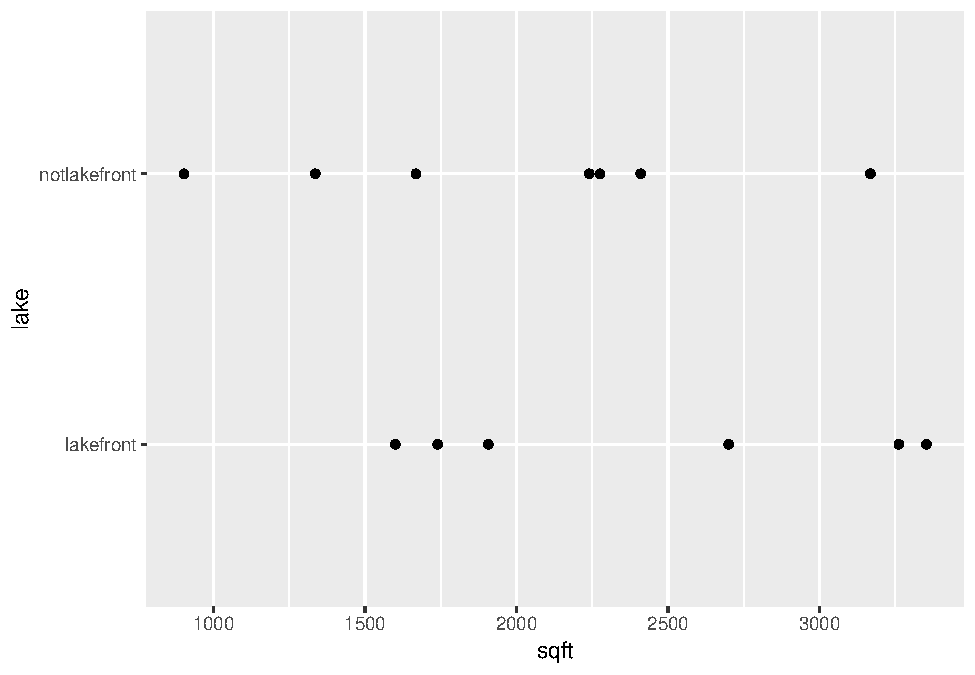
\includegraphics{Michigan_Home_Prices_files/figure-latex/unnamed-chunk-10-1.pdf}

\begin{Shaded}
\begin{Highlighting}[]
\NormalTok{home.data }\OperatorTok
\StringTok{  }\KeywordTok{ggplot}\NormalTok{(}\KeywordTok{aes}\NormalTok{(}\DataTypeTok{x=}\NormalTok{price.}\DecValTok{1000}\NormalTok{,}\DataTypeTok{y=}\NormalTok{lake)) }\OperatorTok{+}
\StringTok{  }\KeywordTok{geom_point}\NormalTok{()}
\end{Highlighting}
\end{Shaded}

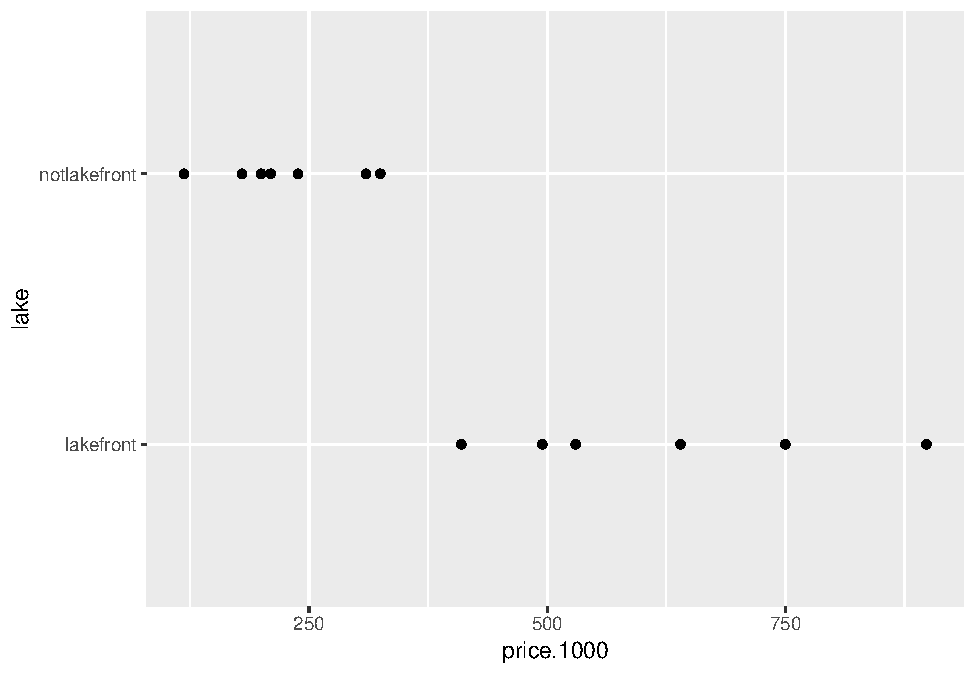
\includegraphics{Michigan_Home_Prices_files/figure-latex/unnamed-chunk-10-2.pdf}

SOLTUION: Location DOES NOT appear to be confounded with home size;
however, there does appear to be a relationship between location and
price of the home (based on both scatter plots).

SOURCES OF VARIATION DIAGRAM: OBSERVED VARIATION IN: Home Prices
INCLUSION CRITERIA: Homes north of Lake Macatawa, Michigan in 2015
SOURCES OF EXPLAINED VARIATION: Home Size (square footage), Location
(Lake Front or Not Lake Front) SOURCES OF UNEXPLAINED VARIATION: Number
of bed/baths, plot size, age of home

\section{Step 4: Draw Inferences beyond the
data}\label{step-4-draw-inferences-beyond-the-data}

Coming in later chapters

\section{Step 5: Formulate
conclusions}\label{step-5-formulate-conclusions}

\begin{enumerate}
\def\labelenumi{\arabic{enumi}.}
\setcounter{enumi}{16}
\tightlist
\item
  Summarize the conclusions of the study, including the statistical
  model I would recommend. Is there a larger population of homes you are
  willing to generalize? Is it reasonable to conclude that either the
  size of the home and/or location of the property is causing variation
  in home prices?
\end{enumerate}

SOLUTION: I would summarize by using the statistical model that includes
location and home size, as this model explained more variance than the
other models considered in the study. My conclusion is that location and
home size has a positive impact on the home price - lake front
properties are generally going to be more expensive and the larger the
home on the lakefront will increase the property value. I would not be
willing to generalize this study to a larger population of homes, as
there are many other factors that could explain variability in home
prices, such as school districts, location to major cities, etc. In this
study, home size and location are extremely likely to cause variation in
home prices.

\begin{enumerate}
\def\labelenumi{\arabic{enumi}.}
\setcounter{enumi}{17}
\tightlist
\item
  Identify any limitation you see to this study. What additional data
  would you like to collect to answer this research question?
\end{enumerate}

SOLUTION: Information about homes in other areas would be particularly
useful to this study, as this study only accounts for two possible
explanations of variations and is very specific to the Lake Macatawa
area.


\end{document}
